\chapter{Software Architecture Design}
\label{ch:software-architecture-design}

This chapter presents the architectural and algorithmic foundation of the proposed EEG-based Motor Imagery (MI) classification system utilizing Self-Supervised Learning (SSL). The system is designed to streamline research workflows involving the acquisition and preprocessing of EEG signals, training of SSL models, and evaluation of model performance on downstream classification tasks.

The architecture adopts a modular and extensible design to ensure compatibility with multiple EEG datasets and learning paradigms, with emphasis on reproducibility, reusability, and interpretability. This chapter details both the algorithmic pipeline and the core artificial intelligence (AI) components used to implement the system.


\section{Domain Model}
\label{sec:domain-model}

The domain model captures the core functional entities involved in the EEG-based Motor Imagery (MI) classification pipeline. Each component reflects a major stage in the self-supervised learning (SSL) research process, from dataset ingestion to performance visualization. This abstraction is not implementation-specific but defines the roles and interactions between major system responsibilities.

\begin{itemize}
    \item \textbf{DataLoader:} Provides access to EEG datasets by parsing files and formatting metadata for downstream processing. It is the system’s entry point for raw input.
    \item \textbf{PreprocessingPipeline:} Encapsulates signal preprocessing operations, such as bandpass filtering, ICA (Independent Component Analysis), normalization, and data segmentation.
    \item \textbf{SSLTrainer:} Manages model setup and training using self-supervised strategies. It supports architecture configuration and model persistence.
    \item \textbf{ModelEvaluator:} Evaluates trained models by computing statistical performance metrics and generating evaluation reports.
    \item \textbf{Visualizer:} Converts numeric evaluation results into visual output formats, including plots, heatmaps, and summary reports.
    \item \textbf{UserInterface:} Acts as the main interaction layer for the researcher, coordinating data upload, model configuration, training initiation, and result export.
\end{itemize}

\begin{figure}[h!]
    \centering
    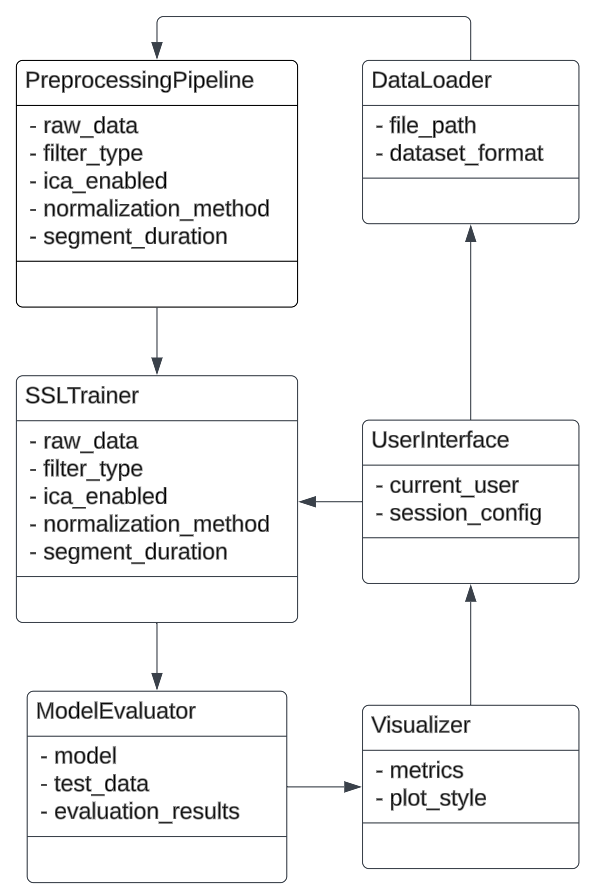
\includegraphics[width=0.5\textwidth]{figures/architecture/domain-model-eeg}
    \caption{Updated Domain Model Corresponding to System Architecture}
    \label{fig:figure9}
\end{figure}

\newpageafter


\section{Design Class Diagram}
\label{sec:design-class-diagram}

The design class diagram formalizes the system's software architecture by mapping each conceptual component from the domain model into its corresponding class with explicit attributes and operations. The architecture is object-oriented and modular, designed for reuse, scalability, and separation of concerns.

\begin{itemize}
    \item \textbf{DataLoader}
    \begin{itemize}
        \item \textit{Attributes:} \texttt{file\_path}, \texttt{dataset\_format}
        \item \textit{Methods:} \texttt{load\_dataset(file\_path: str) $\rightarrow$ EEGDataset}, \texttt{parse\_metadata() $\rightarrow$ dict}
    \end{itemize}

    \item \textbf{PreprocessingPipeline}
    \begin{itemize}
        \item \textit{Attributes:} \texttt{raw\_data: EEGDataset}, \texttt{filter\_type: str}, \texttt{ica\_enabled: bool}, \texttt{normalization\_method: str}, \texttt{segment\_duration: float}
        \item \textit{Methods:}
        \begin{itemize}
            \item \texttt{apply\_bandpass\_filter(low\_freq: float, high\_freq: float) $\rightarrow$ EEGDataset}
            \item \texttt{perform\_ICA(components: int) $\rightarrow$ EEGDataset}
            \item \texttt{normalize(method: str) $\rightarrow$ EEGDataset}
            \item \texttt{segment\_data(duration: float) $\rightarrow$ list[EEGDataset]}
            \item \texttt{preprocess\_all() $\rightarrow$ EEGDataset}
        \end{itemize}
    \end{itemize}

    \item \textbf{SSLTrainer}
    \begin{itemize}
        \item \textit{Attributes:} \texttt{raw\_data: EEGDataset}, \texttt{filter\_type: str}, \texttt{ica\_enabled: bool}, \texttt{normalization\_method: str}, \texttt{segment\_duration: float}
        \item \textit{Methods:}
        \begin{itemize}
            \item \texttt{initialize\_model(architecture: str, task: str) $\rightarrow$ None}
            \item \texttt{train\_model(data: EEGDataset) $\rightarrow$ Model}
            \item \texttt{save\_model(path: str) $\rightarrow$ None}
            \item \texttt{get\_model\_summary() $\rightarrow$ str}
        \end{itemize}
    \end{itemize}

    \item \textbf{ModelEvaluator}
    \begin{itemize}
        \item \textit{Attributes:} \texttt{model: Model}, \texttt{test\_data: EEGDataset}, \texttt{evaluationResults: dict}
        \item \textit{Methods:}
        \begin{itemize}
            \item \texttt{validateOutput() $\rightarrow$ bool}
            \item \texttt{computeMetrics() $\rightarrow$ dict}
            \item \texttt{storeResults(path: str) $\rightarrow$ void}
            \item \texttt{getReport() $\rightarrow$ EvaluationReport}
        \end{itemize}
    \end{itemize}

    \item \textbf{Visualizer}
    \begin{itemize}
        \item \textit{Attributes:} \texttt{metrics: dict}, \texttt{plot\_style: str}
        \item \textit{Methods:}
        \begin{itemize}
            \item \texttt{plotMetrics(metrics: dict) $\rightarrow$ Image}
            \item \texttt{summarizeResults(metrics: dict) $\rightarrow$ str}
            \item \texttt{displayHeatmap(data: EEGDataset) $\rightarrow$ Image}
            \item \texttt{generateReportCard(report: EvaluationReport) $\rightarrow$ str}
        \end{itemize}
    \end{itemize}

    \item \textbf{UserInterface}
    \begin{itemize}
        \item \textit{Attributes:} \texttt{current\_user: Researcher}, \texttt{session\_config: dict}
        \item \textit{Methods:}
        \begin{itemize}
            \item \texttt{uploadData(path: str) $\rightarrow$ void}
            \item \texttt{configureModel(architecture: str, task: str, epochs: int) $\rightarrow$ void}
            \item \texttt{startTraining() $\rightarrow$ void}
            \item \texttt{viewResults() $\rightarrow$ void}
            \item \texttt{exportSession(path: str) $\rightarrow$ void}
        \end{itemize}
    \end{itemize}
\end{itemize}


\begin{figure}[h!]
    \centering
    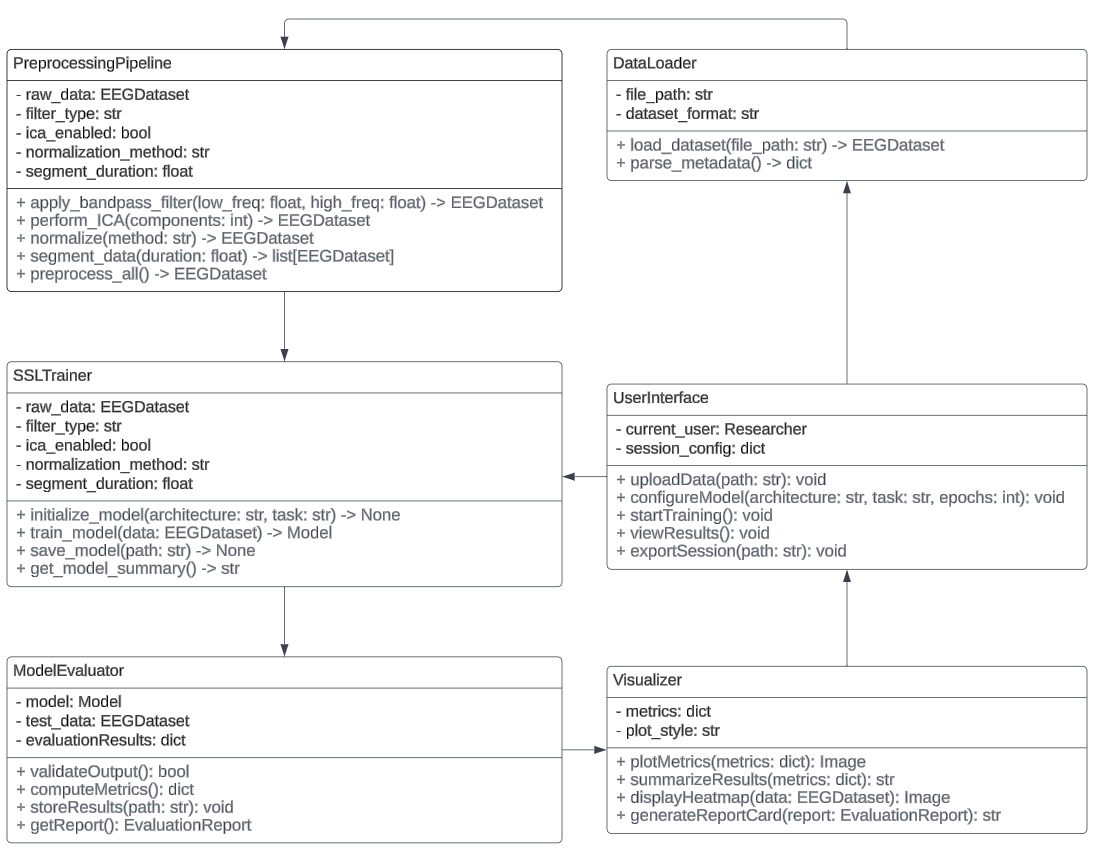
\includegraphics[width=0.75\textwidth]{figures/architecture/design-class-diagram-eeg}
    \caption{Design Class Diagram – Software Architecture of the EEG SSL System}
    \label{fig:design-class}
\end{figure}


\section{Sequence Diagram}
\label{sec:sequence-diagram}

The following sequence diagram illustrates the typical interaction for training a new SSL model on a selected EEG dataset:

\textbf{Scenario: SSL Model Training Workflow}
\begin{enumerate}
    \item Researcher selects and uploads EEG data.
    \item The system applies preprocessing to the dataset.
    \item SSL model is initialized with pretext task configurations.
    \item Training begins, and progress is logged.
    \item Evaluation metrics are computed and visualized.
\end{enumerate}

\begin{figure}[h]
    \centering
    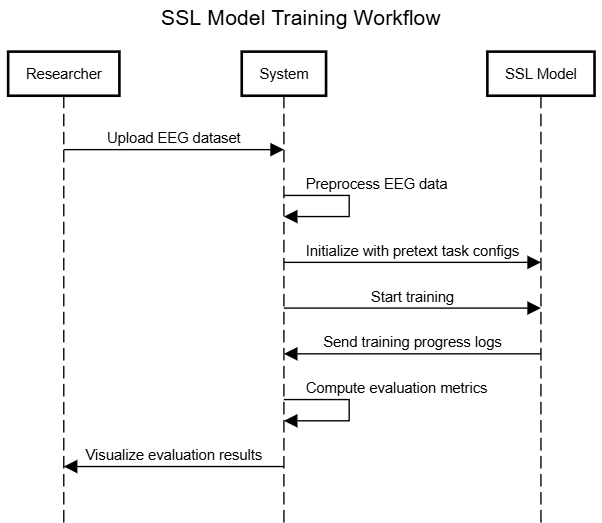
\includegraphics[width=0.75\textwidth]{figures/architecture/sequence-diagram-ssl-eeg}
    \caption{Sequence Diagram – SSL Model Training Flow}
    \label{fig:figure8}
\end{figure}
\newpage


\section{Algorithm}
\label{sec:algorithm}

At the heart of the proposed system lies a contrastive self-supervised learning algorithm tailored for time-series EEG data. The algorithm is designed to leverage large volumes of unlabeled EEG recordings to learn robust and generalizable feature representations that can be transferred to downstream motor imagery classification tasks.

The following pseudocode outlines the main loop of the SSL training process. The approach employs two augmented versions of the same EEG sample to learn invariant representations through contrastive loss optimization.

\begin{verbatim}
Algorithm 1: Self-Supervised EEG Feature Learning
Input: Unlabeled EEG dataset X
Output: Latent representations Z

for epoch in range(num_epochs):
    for batch in X:
        x1, x2 = Augment(batch)
        z1 = Encoder(x1)
        z2 = Encoder(x2)
        loss = ContrastiveLoss(z1, z2)
        UpdateWeights(loss)
\end{verbatim}

\noindent
Each input sample is augmented into two correlated views ($x_1$, $x_2$), which are passed through a shared encoder network to produce latent vectors ($z_1$, $z_2$). The contrastive loss (e.g., InfoNCE or triplet loss) is minimized to bring the representations of positive pairs closer in the embedding space while pushing apart dissimilar (negative) pairs. This process is repeated across multiple epochs to refine the representation space.

Key components of this algorithm include:
\begin{itemize}
    \item \textbf{Data Augmentation:} Introduces semantic-preserving distortions to encourage invariant representation learning.
    \item \textbf{Encoder Network:} Extracts high-level spatiotemporal features from raw EEG signals.
    \item \textbf{Contrastive Objective:} Maximizes similarity between augmentations of the same signal while minimizing similarity with others in the batch.
\end{itemize}


\section{AI Component}
\label{sec:ai-component}

The AI component of the system encapsulates the neural architecture and training pipeline used for self-supervised representation learning. It is inspired by contrastive learning frameworks successfully applied in computer vision (e.g., SimCLR) and adapted to suit the structure and variability of EEG signals.

\subsection*{1. Encoder Network}

The encoder serves as the backbone of the system and is responsible for mapping raw EEG signals into a lower-dimensional latent space. The encoder is designed using convolutional neural networks (CNNs) with architecture modifications to handle EEG's temporal and spatial characteristics.

Supported encoder options include:
\begin{itemize}
    \item \textbf{EEGNet:} A lightweight and efficient CNN architecture widely used in EEG decoding.
    \item \textbf{Custom CNNs:} Deeper networks such as ResNet-18 variants adapted for 1D EEG input.
\end{itemize}

\subsection*{2. Pretext Task Module}

To facilitate self-supervised learning, the system implements multiple pretext tasks—unsupervised objectives that encourage the encoder to learn meaningful features. Each task simulates a predictive learning signal in the absence of labels.

Implemented pretext tasks:
\begin{itemize}
    \item \textbf{Spectral Band Masking:} Randomly suppresses certain EEG frequency bands (e.g., alpha, beta) to enforce frequency robustness.
    \item \textbf{Temporal Shuffling:} Alters the chronological order of EEG segments to encourage temporal sensitivity.
    \item \textbf{Channel Dropout:} Simulates missing sensor data by masking entire EEG channels during training.
\end{itemize}

\subsection*{3. Projection and Loss}

The output of the encoder is passed through a small projection head (typically a two-layer MLP), which maps features into a contrastive embedding space. The contrastive loss then computes the similarity between paired features to optimize learning.

\begin{itemize}
    \item \textbf{Loss Function:} The system supports both InfoNCE and triplet loss:
    \begin{itemize}
        \item \textbf{InfoNCE:} Encourages alignment of positive pairs via a temperature-scaled softmax function.
        \item \textbf{Triplet Loss:} Uses anchor-positive-negative tuples to directly model relative distance constraints.
    \end{itemize}
    \item \textbf{Optimization:} Models are trained using the Adam optimizer with learning rate scheduling and early stopping.
\end{itemize}

\subsection*{4. Fine-Tuning Strategy}

Once the encoder is pretrained on unlabeled EEG datasets using SSL, the learned representations are transferred to a downstream supervised classifier. The classifier is trained on labeled motor imagery tasks to evaluate the quality and transferability of SSL-derived embeddings.

Two fine-tuning approaches are supported:
\begin{itemize}
    \item \textbf{Frozen Encoder:} Only the classifier head is trained while the encoder weights remain fixed.
    \item \textbf{End-to-End Fine-Tuning:} All layers are updated using labeled data to maximize performance.
\end{itemize}

\subsection*{5. Multi-Dataset Support}

To ensure generalizability, the architecture supports training on multiple publicly available datasets (e.g., BCIC2a, OpenBMI, BNCI). The system incorporates a preprocessing pipeline to normalize data across datasets and ensure input compatibility across different recording standards.